\chapter{Introduction}
\label{chapterIntro}
\hl{+Intro EMPOWER/INVADE?} \\
\hl{Energy Policy}
\hl{Regulation from EU and Directives} \\


\section{Smart grids}
\hl{+Definition of smart grid}

The current technical developments in distributed generation can cause bidirectional power flows in grids. Additionally, storage and electric vehicle technologies can create significant variations in household load profiles as shown in Fig. \ref{fig:IntroTesla} and consequently in distribution grids if this technology becomes popular as it is today. This fact has major implications in the power system, from the network planning and regulation to the daily basis grid operation. 

\begin{figure}
	\centering
	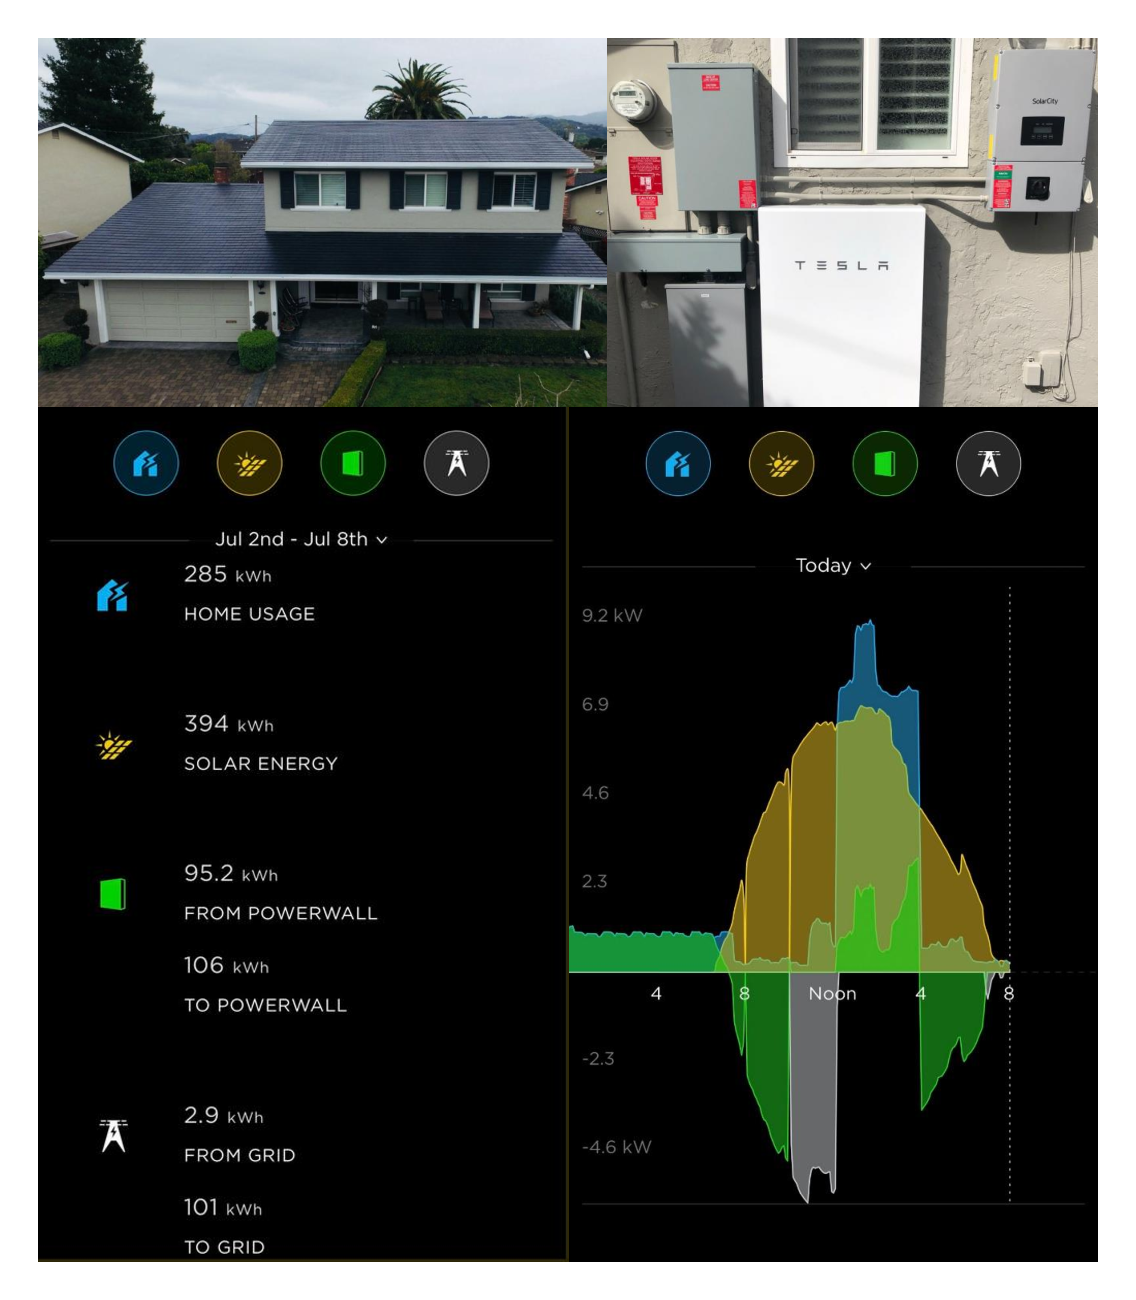
\includegraphics[width=0.8\textwidth]{ChapterIntro/figures/EV_load_profile_Tesla_user.pdf}
	\caption{Household load profile with photovoltaic generation, storage and electric vehicle. Courtesy of \cite{TwitterToblerhaus}}
	\label{fig:IntroTesla}
	\end{figure}

Moreover, the integration of distributed energy resources (DERs) requires smart meters to monitor energy flows, sensors at different levels, and communication technologies to interconnect everything. 
In that sense, cloud-based platforms are clearly a technology that can help power systems operation to solve these issues as it enables to use decision-making algorithms and send control signals based on optimization problems, artificial intelligence and forecasting algorithms.

%Fig. \ref{fig:smart_grid_elements} shows the smart grid elements cited previously. There are four activities that changes from the current power system: production with distributed generators, trading with smart meters data, storage units, flexible demand like electric vehicles and smart homes. 
%
%\begin{figure}
%	\centering
%	\includegraphics[width=0.8\textwidth]{ChapterIntro/figures/smart_grid_elements}
%	\caption{Smart grids elements. Source: \cite{EEGI2010}.}
%	\label{fig:smart_grid_elements}
%\end{figure}
%
%Fig. \ref{fig:smart_grid_view} gives another view of smart grid technologies implementation. It shows distributed electricity and thermal storage units, distributed renewable generators, AC and DC transmissions systems, microgrids and a hydrogen station. Furthermore, the communication infrastructure connects all elements of smart grid.
%
%\begin{figure}[h!]
%	\centering
%	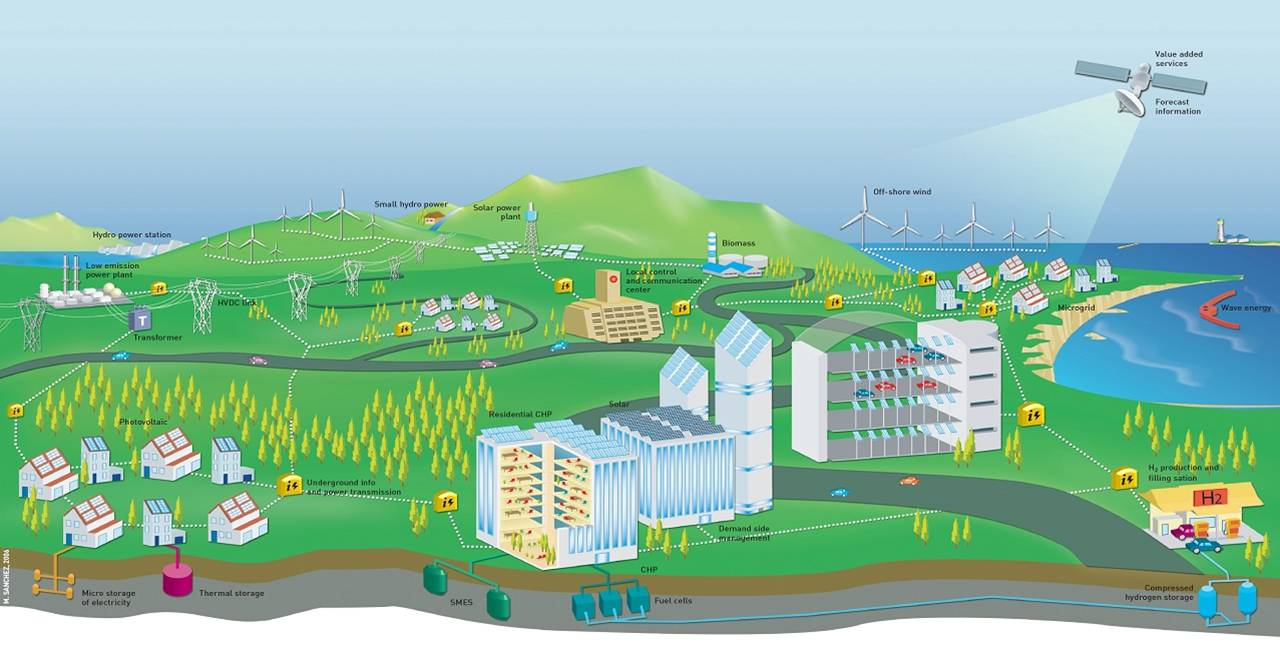
\includegraphics[scale=0.5]{ChapterIntro/figures/smart_grid_vision}
%	\caption{Future network vision of the smart grids. Source: European Technology Platform for the Electricity Networks of the Future \cite{ETP_SG2006}}
%	\label{fig:smart_grid_view}
%\end{figure}

\subsection{Distributed energy resources}
Distributed generation (DG) is based on small but many generators dispersed in the territory. DG moves the consumption closer to production reducing the losses in the grid. 
There are two types of DG: dispatchable and non-dispatchable generators in function of their resource.

The most popular DG technology is the photovoltaic (PV) and this is basically non-dispatchable because it depends on the solar radiation. 
However, recent developments in technology, and more complex grid constraints and market conditions created the need of reducing power generation under certain circumstances.

One of the key factors for DG popularization is its cost-effectiveness for small scale systems and the national level economic incentives.
%Economy of scale
The economic feasibility of an energy generation project can be evaluated using the levelised cost of energy (LCOE) is the most often used. LCOE permits to compare technologies considering all costs of these during their lifespan. The equation \ref{eq:LCOE} is the definition of LCOE and Lazard \cite{Lazard2014} presented this study to compare the costs of them in 2014.
%Feed-in-Tariffs

\begin{equation}
LCOE = \frac{\sum_{t=0}^{T} \frac{I_t+O_t+M_t+F_t}{(1+r)^t}}{\sum_{t=0}^{T} \frac{E_t}{(1+r)^t}}
\label{eq:LCOE}
\end{equation}

\begin{itemize}
	\item $T$: life of the project [years]
	\item $t$: Year
	\item $E_t$: Energy produced for t [$\$$]
	\item $I_t$: Initial investment/cost of the system including construction, installation, etc. [\textdollar]
	\item $O_t$: Operation costs for t [\textdollar]
	\item $M_t$: Maintenance costs for t [\textdollar]
	\item $F_t$: Interest expenditures for t [\textdollar]
	\item $r$: Discount rate for t [$\%$]
\end{itemize}

\begin{table}
	\centering
	\label{Unsubsidised levelised cost of energy comparison. Source: \cite{Lazard2018}}
	\begin{tabular}{lll}
		\textbf{Renewable energy sources} & \textbf{Min} & \textbf{Max} \\ \hline
		Solar PV - Rooftop residential & 160 & 267 \\
		Solar PV - Commercial and community & 73 & 170 \\
		Wind & 29 & 56 \\ \hline
		\textbf{Conventional energy sources} & \textbf{Min} & \textbf{Max} \\ \hline
		Gas peaking & 152 & 206 \\
		Nuclear & 112 & 189 \\
		Coal & 60 & 143 \\
		Gas combined cycle & 41 & 74 \\ \hline
	\end{tabular}
\end{table}

+Review DSO Optimization paper
\subsubsection{Electric vehicles}
+Introduction EVABM paper
\subsubsection{Distributed generation}
Distributed generation is sky-rocketing as their costs plummet.
 
\subsubsection{Batteries}


\subsection{Energy management optimization}
+Review ADMM paper
The advantage of cloud servers for taking decisions

\section{Electricity markets}

\subsection{European and national level markets}
\subsubsection{Day-ahead}
\subsubsection{Intraday}
\subsubsection{Balancing markets}
\hl{+Book chapter}
\hl{Figures Sandro about balancing market price increase}

\subsubsection{Price volatility}
\hl{Episode 7/5/2019 8 pm in Spain. Day-ahead market presentation}
\hl{Episode 2013. Zero prices and high balancing prices}

\subsection{Local electricity markets}
+Review LFM paper
The advantage of being local -> distribution grids congestions
The advantage of being flexible -> Price surfing

\newpage 
\section{Objectives and scope}
This Section presents the objectives and scope of the work conducted by the author during the realisation of this thesis. 
	
	
	This Section presents the objectives and scope of the work conducted by the author during the realisation of this thesis. 
	Fig.~\ref{fig0} depicts a conceptual overview of a number of HVDC systems used to interconnect different countries and to integrate offshore wind power. Submarine cables are assumed for the interconnections and two voltage levels for the HVDC systems are considered: Low Voltage (LV) HVDC and High Voltage (HV) HVDC. The wind turbines represent OWPPs that are interconnected by means of HVDC systems and the different converter topologies are depicted with coloured boxes. The AC grid is not illustrated but it is assumed to be present in the mainland. The previous figure serves as a roadmap to introduce the different topics that have been analysed throughout this thesis. 
	
	Firstly, the modelling and control of a 3-port interline DC/DC Current Flow Controller is analysed \circled{1} and the increase in the operational range that it provides is also investigated. Then, this work continues by proposing an additional 3-port interline DC/DC CFC topology to regulate the current flows with a reduced number of switches \circled{1}. The previous CFC topology is used as a building block to develop the concept of distributed CFC devices with a simplified structure that are installed in different nodes of the grid and that are being operated selectively \circled{2}. Afterwards, the thesis proposes a multi-port CFC converter structure that can be connected to any number of lines, which is based on the previous CFC topology \circled{3}. Taking into account that DC Circuit Breakers (DCCB) are going to be required in HVDC grids, this thesis presents the idea of integrating the CFC capability into the DCCB design, obtaining a device able to provide both functionalities \circled{4}. Focusing on the interconnection of HVDC lines with different voltage level, this thesis also investigates a DC/DC converter for high power and high voltage applications which is based on the autotransformer concept, where the transformer has been substituted for an AC filter. This converter can also be used to control the power flow between the lines where it is connected \circled{5}. Finally, the operation and control of a tapping station based on a Current Source Converter of an LCC-HVDC link is investigated. The previous device shares some features with CFCs as it is also connected in series and applies a variable voltage source, though it is used to integrate offshore wind power \circled{6}.
	

After introducing the topics analysed in the thesis, the objectives and scope are described below:

\begin{itemize}
	\item \textbf{Analyse the impact of electric vehicles in distribution grids, electricity day-ahead markets and buildings}. Electric vehicles will represent a significant new load which is necessary to consider in advance due to their electricity consumption, high shifting capability potential and significant actors involved around the new transportation technology.
	Create a methodology to estimate the EV charging demand in multiple scenarios, create a methodology to analyse distribution grids and electricity markets. Finally, design an EV charging management system for buildings in real environments.
	
	\item \textbf{Design and analyse a flow-based local energy market for interacting with day-ahead markets}. In order to be capable of taking advantage of price volatility, this market design is focused on scheduling local distributed energy resources without threatening the distribution grid.
	
    \item \textbf{Design a local flexibility market for aggregators managing a portfolio of distributed energy resources}. With the introduction of the new market agent called aggregator which aims to schedule flexible resources, the main purpose was to create a market-based framework to fairly manage devices of multiple varied owners. Therefore, each prosumer can settle different flexibility prices through contracts and their activation would depend on the location, flexibility request, availability and price.
      	
	\item \textbf{Build an optimization model based on the local flexibility market framework previously defined to schedule flexibility devices for meeting distribution system operator flexibility requests}. Under the assumption that DSOs could benefit of activating flexibility to deal with congestions in their networks, the objective is to present an optimization model for aggregators which receive the commitment of increasing or decreasing the load in a certain zone. 
	
	\item \textbf{Build an optimization algorithm of flexibility services provision for aggregators remotely managing prosumers}. The optimization model is extended in order to consider the prosumer's behind-the-meter constraints. 
	
	\item \textbf{Build a distributed flexibility provision algorithm for large-scale portfolios}. Additionally, the model uses a decomposition technique in order to reduce the computational burden and time. Such algorithms have to provide a suitable solution in less than 10 minutes and centralized optimization algorithms could have scalability limitations.	
	
\end{itemize}

\newpage 
	\section{Work and activities during the thesis period}
	
	This section provides an overview of the chronological activities developed by the author during the thesis period, both the ones included and non-included in the thesis document.
	
	The predoctoral activities started in March 2014 with a project with Alstom Grid (currently GE). The work consisted on the development of a current flow controller topology for the regulation of DC currents in meshed HVDC grids. The outcomes of that project were two patents filed [P1], [P2] and two journal papers were later published [J1], [J2]. Also, later on a conference paper [C3] related to [J1] was published.
	
	During 2014 the project ENE2013-47296-C2-2-R (``Offshore wind power plants integration in the Spanish electrical system by multi-terminal HVDC links") started, which was funded by the Spanish Ministry of Economy and Competitiveness. The work developed in that project was focused on the integration of offshore wind power plants by means of a bidirectional tapping station of an HVDC link. From this work a conference paper [C1] and a journal paper [J4] were published, which are both part of this thesis. Another journal paper [J8] was published focused on the optimal operation of hybrid AC/DC grids, which is not included in the thesis.
	
	The author participated in a project related to the state of the art of the superconductor cables during 2015. The project was funded by Red El\'{e}ctrica de Espa\~{n}a (Spanish TSO). The results of this project are not part of this thesis.
		 
	In 2016, the project ENE2015-67048-C4-1-R funded by the Spanish Ministry of Economy and Competitiveness started, whose name was ``Breaking technical, economical and regulatory barriers for the development of DC Supergrids". From this work a conference paper was obtained [C2].
	A number of collaborations were conducted with other universities during this period with the respective outcomes: Technical University of Denmark, journal paper [J6], conference paper [C5]; University of Porto, a journal paper [J7]; University of Manchester, a journal paper [J5]. Only, [J5] is part of the thesis. 
	
	The PhD European mobility was carried out from January 2017 to June 2017, at the ABB Corporate Research Center (CRC), V\"{a}ster\r{a}s, Sweden. The author participated in a project to study a transformerless DC/DC converter topology. Form this work, a conference paper [C4] and a submitted journal paper [S-J11] were obtained. 
	
	At the end of 2017, the author participated in a project funded by EIT InnoEnergy, which consisted on testing a three-phase active filter to compensate unbalanced loads and harmonics. This work is not part of the thesis.
	
	In 2017 a scholarship from Fundaci\'{o}n Iberdrola in Spain was obtained to investigate the development of DC/DC converters to regulate the power flows in meshed HVDC grids. From this work, a journal paper was published [J3].
	
	Finally, from the results of project ENE2015-67048-C4-1-R two journal papers were submitted [S-J9] and [S-J10], but only [S-J10] is included in the thesis.
	
	The author is also a member of the EIT InnoEnergy PhD School.
	
	

\newpage 
	\section{Thesis outline}
	
	The contents of the thesis are organized as follows, where each chapter and the appendix A corresponds to one of the objectives of the work:
	
	
	\begin{itemize}
		\item \textbf{Chapter 2} presents the Current Flow Controller concepts that can be found in the literature. The different concepts are gathered and analysed qualitatively.
		
		\item \textbf{Chapter 3} deals with the Dual H-bridge CFC topology, which is a 3-port interline DC/DC converter. The modelling of the converter is provided and its control is designed. The operational area increase is also addressed and simulations are used to validate the designed controllers.
		
		\item \textbf{Chapter 4} integrates the CFC capability of the Dual H-bridge CFC into an Hybrid Circuit Breaker (HCB). The combined circuit is presented and both functionalities are validated. A comparison of the performance of the presented concept and the CFC and the CB in a separate design is also given.
		
		\item \textbf{Chapter 5} introduces a 3-port series interline DC/DC CFC for unidirectional current flows with a reduced number of switches. The modelling and control of the device is presented and then validated using dynamic simulations. The topology is qualitatively compared with the one in Chapter~\ref{chapter1}. Finally, a prototype of the unidirectional CFC is built and tested in the laboratory.
		
		\item \textbf{Chapter 6} presents the concept of Distributed CFC devices installed in different nodes of the HVDC grid that are operated selectively. The Distributed CFC topology is derived from the converter structure from Chapter~\ref{chapter2}.
				
		\item \textbf{Chapter 7} extends the CFC topology presented in Chapter~\ref{chapter2} for a generic number of lines and describes the modelling and the control strategy. It also provides a validation of a 5-port CFC using simulations.
		
		\item \textbf{Chapter 8} describes the Transformerless DC/DC converter topology and analyses and designs the AC filter investigating its effect on the operational limits of the converter.
		
		\item \textbf{Chapter 9} summarises the conclusions of the work and introduces the future research lines for each one of the research topics addressed.
		
		\item \textbf{Appendix A} presents the operation and control of a series tapping station based on a Current Source Converter of an LCC-HVDC link for integrating Wind Power Plants. 
		
		\item \textbf{Appendix B} enumerates the publications related and non-related to the thesis. 
		
	\end{itemize}


